\chapter{Forces}

\section{Types of Forces}

\subsection{Force Fields and Conservative Forces}

\begin{definition}
    A \vocab{force field} is the region of space within which a force is experienced.
\end{definition}

\begin{definition}
    A force is \vocab{conservative} if the work it does on an object moving between two points is independent of the path taken by the object. Else, the force is \vocab{non-conservative}.
\end{definition}

The gravitational force is an example of a conservative force, while friction is an example of a non-conservative force.

\subsection{Tension}

\begin{definition}
    \vocab{Tension} ($T$) is the force exerted by an extended body on another body to which it is attached, and acts along the direction of the extended body.
\end{definition}

\begin{law}[Hooke's Law]
    Within its elastic limit, the magnitude of the tension in an elastic body is directly proportional to its extension.
\end{law}

Mathematically, \[T = kx,\] where $k$ is the spring/force constant and $x$ is the extension.

For a given elastic material, the spring constant $k$ is directly proportional to its cross-sectional area $A$ and inversely proportional to its natural length $l_0$: \[k \propto A \quad \tand \quad k \propto \frac1{l_0}.\]

If two springs of spring constant $k_1$ and $k_2$ are connected in parallel, they can be replaced by a single spring with spring constant \[k_{\text{eff}} = k_1 + k_2.\] If they are connected in series, they can be replaced by a single spring of spring constant \[\frac1{k_{\text{eff}}} = \frac1{k_1} + \frac1{k_2}.\]

\subsection{Normal Contact Forces and Frictional Forces}

\begin{definition}
    A \vocab{contact force} is a force that can only act when objects are physically touching.
\end{definition}

When two solid surfaces are in contact, it is usually possible to represent the forces between them as two components.
\begin{itemize}
    \item \vocab{normal contact forces} that are perpendicular to the surfaces, and
    \item \vocab{frictional forces} that are parallel to the surfaces.
\end{itemize}

Frictional forces are always opposite in the direction to motion.

\subsection{Viscous Forces}

\begin{definition}
    \vocab{Viscous force} is the frictional force experienced by a body when it moves in a fluid. 
\end{definition}

The origin of viscous forces is frictional drag by the fluid and collisions with the displaced molecules of the fluid.

Unlike frictional forces, viscous forces are zero when the body's velocity is zero.

As the relative velocity of the body in the fluid increases, the viscous force on the body increases.

\subsection{Upthrust}

\begin{definition}
    \vocab{Pressure} ($p$) is the normal force per unit area. \[p = \frac{F}{A}.\]
\end{definition}

Pressure is a scalar quantity. Its SI unit is pascal (Pa) or the newton per square metre. Alternate units include the atmosphere (atm), the millimetre of mercury (mmHg) and the bar.

\begin{definition}
    \vocab{Density} ($\rho$) is the mass per unit volume. \[\rho = \frac{m}{V}.\]
\end{definition}

Density is a scalar quantity. Its SI unit is kilogram per cubic metre (kg m$^{-3}$).

\begin{proposition}[Hydrostatic Pressure]
    Consider an object at depth $h$ in a fluid of density $\rho$. The pressure $p$ exerted \emph{by the fluid} on the object is given by \[p = \rho g h.\]
\end{proposition}
\begin{proof}
    By the definitions of pressure and density, we have \[p = \frac{F}{A} = \frac{\text{weight of fluid column}}{A} = \frac{mg}{A} = \frac{\rho V g}{A} = \rho g h.\]
\end{proof}

This implies that pressure is independent of the cross-sectional area of the body and the shape of the container holding the fluid.

If the surface of the fluid is subject to pressure $p_s$ from another fluid, then the pressure $p_s$ should be added: \[p = \rho g h + p_s.\]

\begin{definition}
    \vocab{Upthrust}, $U$ is the vertical upward force exerted by a fluid on a body when the body is (completely or partially) submerged in the fluid.
\end{definition}

Upthrust arises because pressure in a fluid increases with depth, hence pressure on the lower surface is greater than that on the upper surface, resulting in a net upward force.

\begin{principle}[Archimedes' Principle]
    When a body is immersed in a fluid, it experienced an upthrust equal in magnitude to the weight of fluid displaced. Mathematically, \[U = m_f g,\] where $m_f$ is the mass of the fluid.
\end{principle}
\begin{proof}[Justification]
    Consider a cylinder of cross-sectional area $A$ and length $l$ that is submerged in a fluid of density $\rho$.

    The net upward force $U$ is thus given by \[U = \D F = \D (pA) = \D (\rho g h A) = \bp{\rho A \D h} g = \bp{\rho A l} g = \bp{\rho V} g = m_f g.\]
\end{proof}

\begin{principle}[Principle of Floatation]
    When an object is floating in a fluid, the weight of the object is equal to the weight of fluid displaced by the object.
\end{principle}

\section{Turning Effect of Forces}

The motion of a body is made up of translation and rotation. A motion is
\begin{itemize}
    \item purely \vocab{translational} if every particle in the body has the same instantaneous velocity,
    \item purely \vocab{rotational} if every particle is in circular motion about the same axis of rotation.
\end{itemize}

\subsection{Centre of Gravity}

\begin{definition}
    The \vocab{centre of gravity} (C.G.) of a body is the point at which the whole weight of the body may be considered to act.
\end{definition}

\begin{definition}
    The \vocab{centre of mass} of a body is the point at which the mass of the body appears to b concentrated.
\end{definition}

In a uniform gravitational field, the C.G. coincides with the centre of mass.

\subsection{Moment and Torque}

\begin{definition}
    The \vocab{moment} ($M$) of a force $F$ about a pivot point is the product of the force and the perpendicular distance $d$ between its line of action and the pivot point. \[M = F d.\]
\end{definition}

Moment is a vector quantity. Its direction is given by the right-hand rule. Its SI unit is newton-metre (N m).

Intuitively, moment can be thought of as the ability of a force to rotate a body about a given pivot point.

\begin{definition}
    A \vocab{couple} is a pair of forces of equal magnitude but opposite in directions.
\end{definition}

A couple tends to produce rotations only.

\begin{definition}
    The \vocab{torque} ($\tau$) of a couple is the product of one of the forces $F$ and the perpendicular distance $d$ between the forces. \[\tau = F d.\]
\end{definition}

Torque is a vector quantity. Its SI unit is newton metre (N m).

\begin{figure}[H]
    \centering
    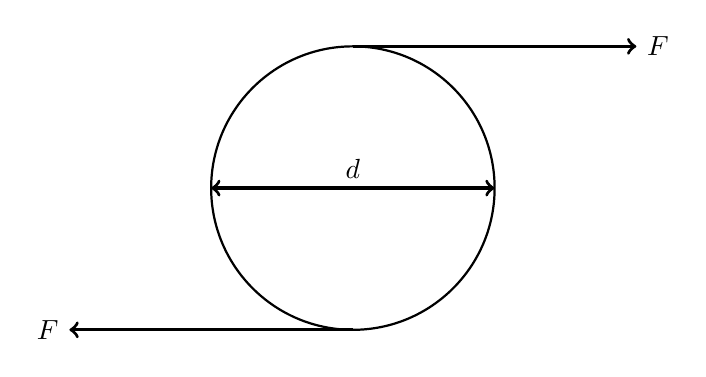
\begin{tikzpicture}[scale=0.6]
        \draw[thick] (0, 0) circle[radius=3];
        \draw[->, very thick] (0, 3) -- (6, 3) node[anchor=west] {$F$};
        \draw[->, very thick] (0, -3) -- (-6, -3) node[anchor=east] {$F$};
        \draw[<->, very thick] (-3, 0) -- (3, 0);
        \node[anchor=south] at (0, 0) {$d$};
    \end{tikzpicture}
    \caption{A couple. The magnitude of the torque is given by $Fd$.}
\end{figure}

Any system of forces acting on a body can usually be reduced to
\begin{itemize}
    \item a single force acting through a point which only affects translational motion, and
    \item a torque (of a couple) which only affects its rotational motion.
\end{itemize}

On their own, the term ``moment'' usually refers to a turning effect of a force, while the term ``torque'' usually refers to a turning effect without translational effect.

\section{Equilibrium of Forces}

\begin{definition}
    \phantom{.}
    \begin{itemize}
        \item A body is in \vocab{translational equilibrium} if the resultant force on it is zero in all directions.
        \item A body is in \vocab{rotational equilibrium} if the resultant torque on it is zero about all axes of rotation.
        \item A body is said to be in \vocab{equilibrium} if it is in both translational and rotational equilibrium.
    \end{itemize}
\end{definition}

\begin{principle}[Principle of Moments]
    When a system is in equilibrium, the sum of clockwise moments about any axis must be equal to the sum of anti-clockwise moments about the same axis.    
\end{principle}

If three (non-parallel) forces result in equilibrium, then their lines of action share a common point.

\begin{figure}[H]
    \centering
    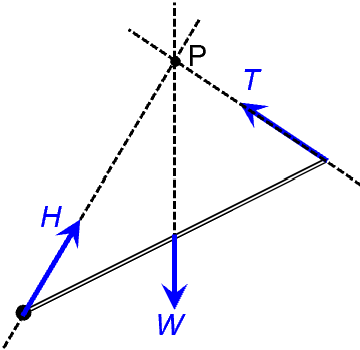
\includegraphics[scale=0.4]{media/Equilibrium.png}
    \caption{The lines of action of $H$, $T$ and $W$ intersect at a common point $P$.}
\end{figure}